%\documentclass[11pt,a4paper,twocolumn]{article}
\documentclass{svmult}

\usepackage{makeidx}         % allows index generation
\usepackage{graphicx}        % standard LaTeX graphics tool
                             % when including figure files
\usepackage{multicol}        % used for the two-column index
\usepackage[bottom]{footmisc}% places footnotes at page bottom

%\usepackage{msk}
\usepackage[english]{babel}
\usepackage[cp1250]{inputenc}
\usepackage[OT4]{fontenc}
%\usepackage{graphicx}
%\usepackage{indentfirst}
\usepackage[urlcolor=black,colorlinks=false,bookmarks=true,bookmarksnumbered=true]{hyperref}


\title{\emph{Salomon} -- %komponentowa architektura indukcyjnej bazy
  %danych jako platformy uczenia maszynowego}
  Component-based Architecture of Inductive Database as a Machine Learning Platform}

\author{
 Krzysztof Rajda\inst{1}
 Nikodem Jura\inst{1} %\and
 Marek Kisiel-Dorohinicki\inst{1} %\and
 Bart�omiej �nie�y�ski\inst{1}}
\authorrunning{Salomon}
\titlerunning{Salomon}

\institute{AGH University of Science and Technology, Institute of
Computer Science, Krak\'ow, Poland\\
\href{mailto:nico@icslab.agh.edu.pl}{nico@icslab.agh.edu.pl},
\href{mailto:krzysztof@rajda.name}{krzysztof@rajda.name},
\href{mailto:doroh@agh.edu.pl}{doroh@agh.edu.pl},
\href{mailto:sniezyn@agh.edu.pl}{sniezyn@agh.edu.pl}}


\begin{document}

\maketitle

\begin{abstract}
%Nowym kierunkiem ��cz�cym technologie baz danych z nowoczesnymi
%metodami indukcyjnego generowania wiedzy s� indukcyjne bazy
%danych.
Inductive database is a new direction which merges database
technology with inductive methods of knowledge generation.
% Po��czenie takie pozwala na jednolity dost�p do wiedzy
%zawartej w~danych bezpo�rednio i wiedzy wygenerowanej z tych
%danych za pomoc� algorytm�w uczenia maszynowego.
This merging allows to access to the knowledge and data in a
consistent manner, e.g. using machine learning algorithms.
% W~niniejszej
%pracy przedstawiona zosta�a architektura i~wybrane aspekty
%implementacji platformy \emph{Salomon}, komponentowej realizacji
%indukcyjnej bazy danych.
The architecture and chosen aspects of implementation of the
inductive database \emph{Salomon} platform have been presented in
this article.
%Dzi�ki budowie modu�owej uda�o si�
%uzyska� du�o lepsz� elastyczno�� systemu w~stosunku do innych,
%zbli�onych rozwi�za�.
Because of the modular structure, a good flexibility in comparison
to other similar systems is gained.

\end{abstract}

\section{Wprowadzenie}
%\subsection{Machine learning}
%\subsection{Indukcyjne bazy danych}
%\subsection{Zastosowania}

Integracja technologii baz danych z nowoczesnymi metodami indukcyjnego
generowania wiedzy wydaje si� dawa� istotne korzy�ci w perspektywie
budowy system�w wspomaganie decyzji. Systemy nazywane czasem
indukcyjnymi bazami danych potrafi� odpowiedzie� nie tylko na pytania,
dla kt�rych odpowied� znajduje si� w bazie danych, ale r�wnie� na
pytania, kt�re wymagaj� zsyntetyzowania i zastosowania wiarygodnej
wiedzy, wygenerowanej przez indukcyjne wnioskowanie z fakt�w z bazy
danych i wcze�niejszej wiedzy.  Indukcyjne bazy danych mog� by�
postrzegane jako naturalny krok w rozwoju system�w bazodanowych \cite{bib3}.

\begin{figure}[ht]
    \centering
        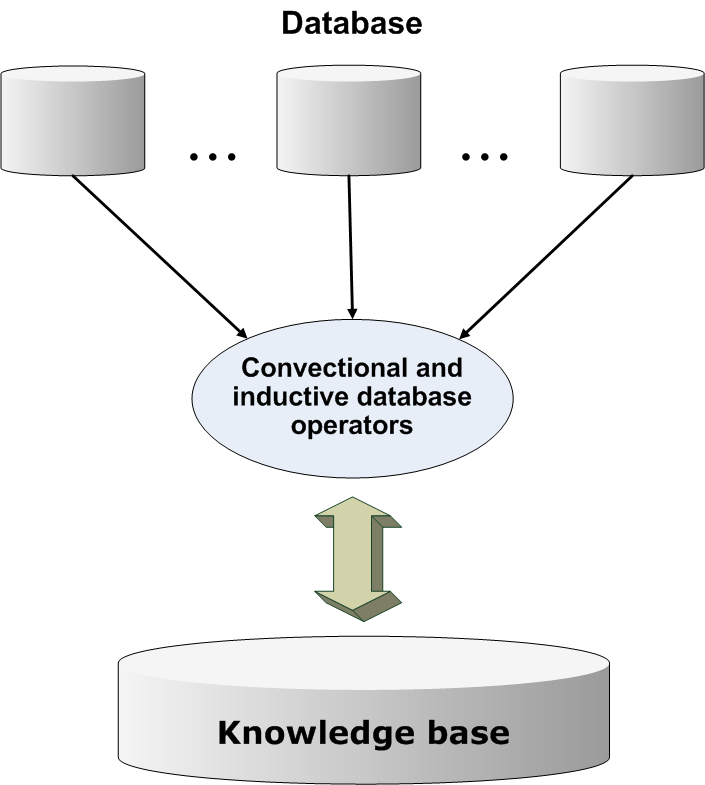
\includegraphics[width=0.70\textwidth]{img/knowledge_mining.png}
    \caption{Indukcyjne bazdy danych}
    \label{fig:architecture}
\end{figure}

\bigskip
W pracy przedstawiona zostanie architektura i wybrane aspekty
implementacji platformy \emph{Salomon}, jak r�wnie� zaprezentowane
zostan� mo�liwo�ci jego wykorzystania na przyk�adzie wybranych
algorytm�w pozyskiwania wiedzy z danych.

%\newpage
\section{Prace pokrewne}

\frame{
	\frametitle{Prace pokrewne}
	\begin{itemize}
		\item Weka
			\begin{itemize}
				\item Narz�dzie do prowadzenia eksperyment�w zwi�zanych z~uczeniem maszynowym
				\item Implementuje wiele r�nych rodzaj�w algorytm�w
				\item Wykorzystywana w zastosowaniach akademickich
			\end{itemize}		
		\item YALE
			\begin{itemize}
				\item R�norodno�� operator�w -- klasyfikuj�ce, klastruj�ce, asocjacyjne, oparte o drzewa decyzyjne
				\item Mo�liwo�� tworzenia ,,�a�cuch�w'' z�o�onych z r�nych problem�w
			\end{itemize}		
		\item Vinlen		
			\begin{itemize}
				\item Prekursor system�w realizuj�cych koncepcj� indukcyjnej bazy danych
				\item Rozwijany na \emph{George Mason University} pod opiek� prof. Ryszarda Michalskiego
			\end{itemize}
	\end{itemize}	
}
\section{Za�o�enia i koncepcja platformy}

\frame{
	\frametitle{Analiza wymaga�}
	\begin{itemize}		
		\item Przyjazny interfejs u�ytkownika
		\item Dobrze zdefiniowany interfejs programistyczny
		\item Odizolowanie algorytm�w od szczeg��w implementacyjnych platformy
		\item Sp�jna reprezentacja wiedzy dla wszystkich algorytm�w
		\item Komponentowa architektura
		\item Wykorzystanie gotowych implementacji algorytm�w
		\item Otwarta licencja \emph{(LGPL)}
	\end{itemize}		
}

\frame{
	\frametitle{G��wne za�o�enia}
	\begin{itemize}
			\item Koncepcja zadaniowo�ci			
			\begin{itemize}
				\item Zadanie -- atomowa jednostka reprezentuj�ca obliczenia
				\item Tworzenie powi�za� mi�dzy zadaniami
			\end{itemize}
    	\item Budowa komponentowa
    	\item Otwarto�� architektury
    	\item Niezale�no�� od �rodowiska wdro�enia
    	\item Prostota u�ytkowania
    \end{itemize}
}


\section{Architektura}

%diagram

System zosta� podzielony na 3 g��wne cz�ci: platform�, kontrolery
i~pluginy.

\begin{figure}[htb]
	\centering
		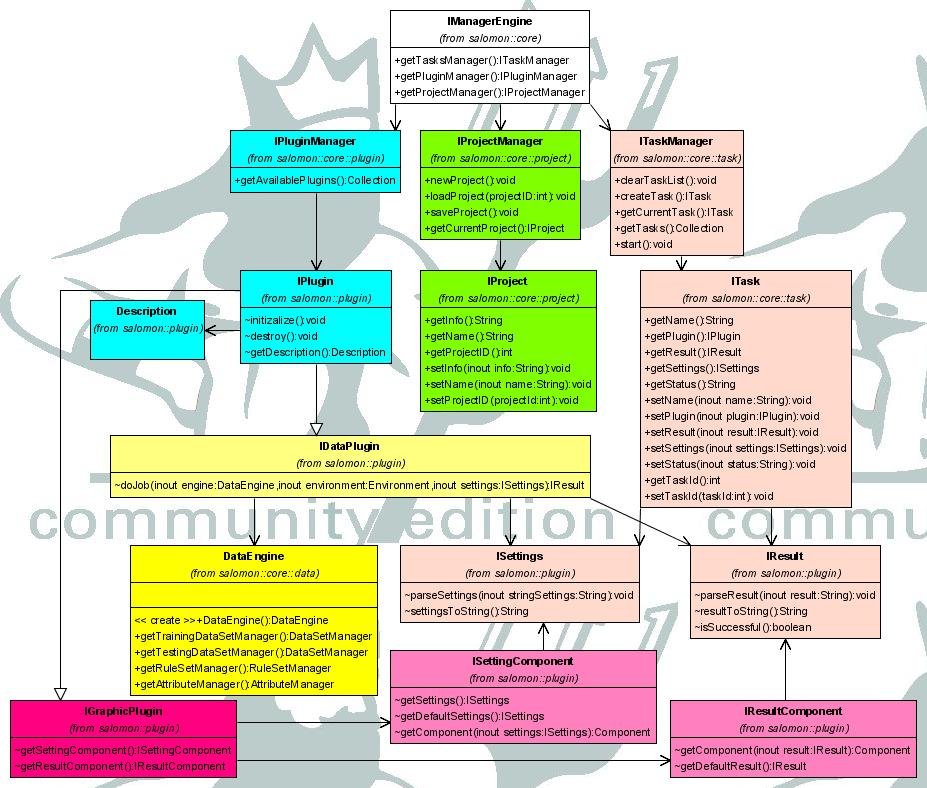
\includegraphics[width=0.90\textwidth]{img/uml/core.jpg}
	\caption{G��wne klasy systemu}
	\label{fig:core}
\end{figure}


\subsection{Platforma}

Dostarcza podstawowej funkcjonalno�ci  umo�liwiaj�cej prac� ca�ego
systemu,  �aduje odpowiedni kontroler, wczytuje pluginy, uruchamia
zadania. Za poszczeg�lne zadania odpowiadaj� odpowiednie menad�ery.

Menad�ery nie s� dost�pne bezpo�rednio z platformy, ale
przekazywane s� pluginom poprzez klas� \emph{DataEngine}. Dotyczy
to tylko klasy \emph{DataSetManager} i \emph{RuleSetManager},
pozosta�e nie s� dost�pne dla plugin�w. Plugin, zale�nie od
potrzeb, pobiera z niego potrzebny mu menad�er i za jego
po�rednictwem wykonuje operacje na bazie danych.

Bardzo wa�nym mechanizmem Salomona jest mo�liwo�� tworzenia powi�za� mi�dzy poszczeg�lnymi zadaniami. Wynik jednego zadania mo�e pos�u�y� jako wej�cie nast�pnego. Salomon w tym celu dostarcza �rodowisko. Wtyczka w trakcie wykonywania zadania opr�cz dost�pu  do manad�er�w posiada r�wnie� dost�p do �rodowiska, z kt�rego mo�e pobra� warto�ci zmiennych �rodowiskowych. Dane �rodowisko tworzone jest na pocz�tku wykonania listy zada� i przekazywane jest kolejno do nast�pnego zadania. Wtyczka w trakcie pracy mo�e modyfikowa� �rodowisko poprzez dodawanie, usuwanie oraz edycj� poszczeg�lnych zmiennych. W ten spos�b poszczeg�lne zadania mog� mi�dzy sob� przekazywa� informacje. Zmienne �rodowiskowe, podobnie jak ustawienia i rezultaty zada�, s� persystentne, a co za tym idzie potrzebny jest mechanizm serializacji i deserializacji.

W obecnej wersji mechanizm ten jest bardzo ubogi  - pozwala on na przekazywanie wy��cznie danych tekstowych. Wraz z pojawieniem si� kolejnej wersji, zmienne �rodowiskowe wykorzystywa� b�d� nowy mechanizm serializacji. Mo�liwo�� tworzenia zmiennych �rodowiskowych przez wtyczki mo�e rodzi� wiele problem�w z zapewnieniem kompatybilno�ci mi�dzy r�nymi wersjami wtyczek, komunikuj�cych si� ze sob�, dlatego te� aby unikn�� takich problem�w, ka�da wtyczka zmuszona b�dzie dostarczy� opis zmiennych, kt�re mo�e tworzy�.

W kolejnej wersji Salomona dodane zostan� klasy odpowiedzialne za przechowywanie danych. Klasy te b�d� odpowiada� poszczeg�lnym typom prostym oraz strukturze (struktura b�dzie mog�a zawiera� inne struktury oraz typy proste). Za pomoc� takich element�w, programista b�dzie m�g� stworzy� hierarchiczne struktury danych. Wprowadzenie takiego mechanizmu podyktowane jest potrzeb� ukrycia przed programist� sposobu zapisu danych w bazie lub w pliku. W obecnej wersji Salomona, tw�rca wtyczki musi dostarczy� mechanizm serializacji oraz deserializacji ustawie� i rezultat�w zada� do napisu � taki mechanizm niesie za sob� niebezpiecze�stwo niepoprawno�ci oraz nieefektywno�ci implementacji. Dostarczenie sp�jnego modelu seralizacji danych pozwala na niewidoczny dla wtyczek spos�b podmiany implementacji na bardziej efektywn� itp. Mechanizm ten mo�e okaza� si� r�wnie� po�yteczny po dodaniu do Salomona mo�liwo�ci definiowania zada� w pliku (np. XML). Seralizacja danych mo�e odbywa� si� do wielu format�w np. XML, CSV, tabel w bazie danych itp. 


\newpage

\subsection{DataEngine}
Klasa przekazywana pluginom podczas ich wykonania.
Za pomoc� pobieranych z niej menad�er�w (\emph{DataSetManager}, \emph{RuleSetManager}, w przysz�o�ci \emph{AttributeManager} i inne) wtyczki mog� operowa� na danych znajduj�cych si� w bazie.

\begin{figure}[htb]
	\centering
		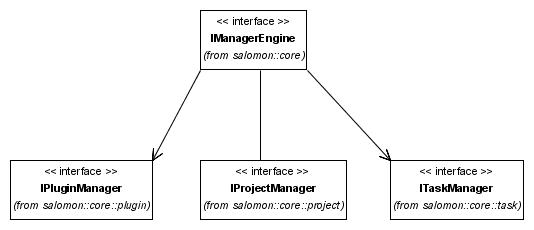
\includegraphics[width=0.80\textwidth]{img/uml/manager_engine.jpg}
	\caption{Interfejsy do zarz�dzania wiedz�}
	\label{fig:manager_engine}
\end{figure}

\subsubsection{DBManager}
Odpowiada za po��czenie z baz� danych. Dostarcza metody
zapewniaj�ce dost�p do danych przechowywanych w bazie. Swoj�
funkcjonalno�� udost�pnia odpowiednim menad�erom.

\subsubsection{DataSetManager}
Zarz�dza zbiorami danych. Pozwala tworzy� nowe podzbiory danych na
podstawie zawartych w bazie informacji oraz umo�liwia operowanie
na nich.
\subsubsection{RuleSetManager}
Zarz�dza regu�ami. Pozwala tworzy� nowe regu�y oraz
zarz�dza dost�pem do ju� istniej�cych.

\newpage

\subsubsection{IManagerEngine}
Klasa zarz�dza pozosta�ymi menad�erami. Utrzymuje jedn� instancj� ka�dego z nich 
i udost�pnia je pozosta�ym klasom z platformy.

\begin{figure}[htb]
	\centering
		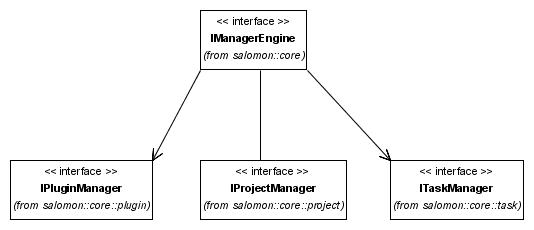
\includegraphics[width=0.90\textwidth]{img/uml/manager_engine.jpg}
	\caption{G��wna klasa zarz�dzaj�ca}
	\label{fig:manager_engine}
\end{figure}

\subsubsection{IProjectManager}
Zarz�dza projektami. Pozwala na utworzenie nowego
projektu, zapisanie bie��cego do bazy danych oraz na za�adowanie z bazy.

\subsubsection{IPluginManger}
Zarz�dza pluginami. Pozwala na utworzenie zapisanie informacji o nowym pluginie (jego nazwa, lokalizacja) oraz na pobranie listy dost�pnych plugin�w.

\subsubsection{ITaskManger}
Zarz�dza zadaniami. 

\subsection{Kontrolery}
Kontrolery odpowiadaj� za interakcj�
systemu z otoczeniem. W zale�no�ci od konfiguracji systemu przy
starcie uruchamiany jest jeden z kontroler�w. Kontrolery operuj�
na danych poprzez wsp�lny interfejs, a co za tym idzie, dane
utworzone poprzez jeden z nich s� dost�pne pomi�dzy kolejnymi
uruchomieniami programu dla pozosta�ych kontroler�w.

\subsubsection{LocalController}
Jest najprostszym kontrolerem. Zarz�dza zadaniami wykonywanymi na lokalnym komputerze. S� one
wykonywane sekwencyjnie. Zadaniem tego kontrolera jest dostarczenie
interfejsu u�ytkownika, pozwalaj�cego na zarz�dzanie projektami,
wtyczkami i zadaniami.

\subsubsection{MasterController}
Zadaniem tego kontrolera jest dostarczenie interfejsu do
zarz�dzania zdalnymi kontrolerami (\emph{ServantController}). Po
uruchomieniu nas�uchuje na po��czenia od klient�w, rozdziela
zadania oraz wy�wietla ich wyniki.

\subsubsection{ServantController}
Zadaniem tego kontrolera jest odszukanie g��wnego kontrolera
(\emph{MasterController}), zarejestrowanie si� i udost�pnianie mu
swoich us�ug. Ta wersja kontrolera nie posiada GUI, zarz�dzanie
nim odbywa si� za pomoc� klasy \emph{MasterController}.


\subsection{Pluginy}
G��wna funkcjonalno�� zosta�a  przeniesiona
do plugin�w, zadaniem systemu jest tylko zarz�dzanie ich
wykonaniem. Dzi�ki takiemu podej�ciu system jest �atwo skalowalny
i rozszerzalny o nowe mo�liwo�ci. Ka�dy z plugin�w musi
implementowa� nast�puj�ce interfejsy:


\subsubsection{IGraphicPlugin}
Pozwala pobra� parametry od u�ytkownika, kt�re nast�pnie zostan�
przekazane do plugin�w  przed ich wykonaniem. Zawiera dwie metody:
\emph{getSettingsPanel()}  i \emph{getResultPanel()}.  Pierwsza z
metod zwraca panel s�u��cy do konfiguracji pluginu, druga � panel,
na kt�rym prezentowane s� wyniki jego dzia�ania.

\subsubsection{IDataPlugin}
Posiada tylko jedn� metod� \emph{doJob()}. Przyjmuje ona jako
parametry obiekt klasy \emph{Environment}, reprezentuj�cy aktualny
stan systemu; \emph{DataEngine}, kt�ry umo�liwia operowanie na
bazie danych i \emph{ISettings}, reprezentuj�cy ustawienia
pluginu. Zwracany jest obiekt klasy \emph{IResult}, stanowi�cy
rezultat wykonania zadania.
\section{Przyk�adowe zastosowanie}

W ramach zaj�� na uczelni, zosta�a podj�ta pr�ba zaimplementowania 
algorytm�w drzew decyzyjnych w oparciu o platform� \emph{Salomon}.

Zgodnie z architektur� systemu, problem zaimplementowany zosta� 
za pomoc� odpowiednich wtyczek, z kt�rych ka�da przeznaczona by�a 
do realizacji osobnego etapu oblicze�.

Zadaniem pierwszej z nich jest konfiguracja procesu przetwarzania 
danych. Pozwala ona na wyb�r cechy, wzgl�dem kt�rej tworzone jest 
drzewo decyzyjne oraz cech, kt�re s� brane pod uwag� przy jego budowie.
Wyb�r ten odbywa si� przy u�yciu graficznego interfejsu u�ytkownika 
i mo�e dotyczy� dowolnej tematyki, zale�nie od danych, na kt�rych 
maj� by� przeprowadzane obliczenia. 
W naszym przypadku na podstawie kilku cech opisuj�cych kandydat�w do pracy, 
takich jak np. wiek, do�wiadczenie zawodowe, znajomo�� j�zyk�w obcych, 
tworzone by�o drzewo maj�ce na celu da� odpowied� na pytanie, 
czy dany kandydat powinien by� zatrudniony.

Druga wtyczka jest w�a�ciw� wtyczk� obliczeniow� -- jej zadaniem jest 
dostarczenie algorytmu, za pomoc� kt�rego tworzone jest drzewo. 
Dla cel�w demonstracyjnych wybrany zosta� jeden 
z najprostszych algorytm�w -- ID3.

Ostatnia wtyczka ma na celu wizualizacj� utworzonego przez 
wtyczk� algorytmiczn� drzewa w celu przedstawienia jej u�ytkownikowi.
W~obecnej wersji drzewo to przedstawiane jest w formie tekstowej, 
jednak�e dzi�ki niezale�no�ci poszczeg�lnych wtyczek od siebie, 
nic nie stoi na przeszkodzie, �eby doda� stworzy� now�, 
kt�ra realizuje wizualizacj� w dowolny inny spos�b.


\section{Case study}
%Rozwa�my sytuacje, kiedy zamierzamy stworzy� system wspomagaj�cy onkolog�w w 
%diagnostyce nowotworowej.Do dyspozycji mamy dane z wielu szpitali rozproszonych 
%po ca�ej Polsce.
Let us consider situations in which we are going to create a system aiding 
oncologists in tumor diagnosis. We have data from  
many hospitals distributed all over entire Poland.
%Ze wzgl�d�w wydajno�ciowych oraz bezpiecze�stwa (szpitale nie 
%wyra�aj� zgody udost�pnianie ich danych innym plac�wk�) nie mo�liwy jest 
%jednoczesny dost�p do wszystkich baz. Naszym celem stworzenie regu� 
%wspomagaj�cych lekarzy przy diagnostyce nowotwor�w. W tym celu przej�li�my 
%nast�puj�ce podej�cie.
Because of the efficiency and the safety constraints (hospitals are not wishing to share their data with other institutions) a 
simultaneous access to all databases is not possible. Our purpose is to create
a set of rules, which aid doctors at the diagnosis of cancer. To achieve 
this purpose we adopted the following approach.
%Szukamy generalnych regu� dla wszystkich przypadk�w 
%(zgodnych z danymi w ka�dej bazie) oraz regu� najbardziej pasuj�cych dla danej 
%plac�wki. Dodatkowo zale�y nam na grupowanie przypadk�w ze wzgl�du na ich 
%zgodno�� do og�lnych regu� (najbardziej, �rednio i najmniej zgodne) i dla 
%ka�dej z tych grup znalezienie bardziej specyficznych regu�. 
We search for general rules for all coincidences (according to 
data in every base) and of rules for the most fitting every institution. 
Additionally, we focus on grouping cases on account of their
agreement to general rules (the most, on average and least agreeable) and for each of these groups finding more unique rules.
% Takie pogrupowanie pozwoli na uproszenie regu� (stan� si�
%czytelniejsze 
%dla lekarzy) dla ka�dej takiej grupy, co pozwoli analitykowi na ewentualne 
%sterowanie procesem uczenia. Dodatkowo chcieliby�my mie� dost�p do danych 
%statystycznych, dla poszczeg�lnych plac�wek (por�wnanie z reszt�).
Grouping coincidences allows to simplify rules (will become more readable 
for doctors) for each such group, which will allow the analyst to 
potentially steer the process of learning. Additionally, we would like to have 
access to statistical data, for individual institutions (comparison to the 
rest).
%Wp�yw r�nych czynnik�w w zale�no�ci o po�o�enia geograficznego, oraz wielko�� 
%poczeg�lnych gr�p. Takie dane nie tylko u�yteczne byby�y dla lekarzy czy os�b 
%steruj�cych procesem odkrywania widzy, ale mog�by by� r�wnie� wykorzystane jako 
%dane wej�ciowe dla algorytm�w uczenia maszynowego.
The influence of different factors in the relation against locations geographical, and size of particular group. 
Such data could be useful not only for doctors or people responsible for steering the process of learning, but they could be used
as the input for algorithms of machine learning.

%%%%%%%%%%%%%%%%%%%%%%%%%%%%%%%
%Przedstawiamy spos� realizacji takiego zadania z wykorzystaniem systemu
%\emph{Salomon}. Obecna wersja nie posiada zaimplementowanych wszystkich
%niezb�dnych funkcjonalno�ci, jednak wszystkie one powinny pojawi� si� w kolejnym
%wydaniu.
We present the way to the realization of such an objective by using 
the system \emph{Salomon}. The current version lacks the implementation of all 
essential functionalities, however they all should available at the next
edition.

%%%%%%%%%%%%%%%%%%%%%%%%%%%%%%%%
%Zgodnie z za�o�eniami zadania, nie mo�liwa jest wymiana danych o pacjentach 
%mi�dzy plac�wkami. Wymaga�oby to stworzenia pot�nego centrum sk�aduj�cego 
%wszystkie dane, albo dost�pu zdalnego do tych danych dla algorytm�w, co jednak 
%z racji ograniczonej przepustowo�ci sieci bardzo spowolni�oby obliczenia.
According to the principles of the objective, an exchange of data about 
patients is not possible among institutions. It would require creating a 
vast centre for storing all data or the remote access to these data for algorithms.
However, a remote access could reduce the speed of computation because of the 
network capacity.
%Dodatkowo tak wielka ilo�� danych jest nie mo�liwa do przeanalizowania w 
%sensownym czasie. Je�li w naszych przyk�adowym zastosowaniu bezpiecze�stwo 
%danych nie jest spraw� krytyczn�, to jednak mo�na sobie wyobrazi� wiele 
%przyk�adowych zastosowa�, dla kt�rych ka�dej plac�wce zale�a�oby na 
%nieudost�pnianiu swoich danych.
Additionally, such amount of data is not possible to be analyzed in a 
sensible time. In our demonstration applying the data security it is not a 
critical matter, however it is possible to imagine a lot 
of example usages, in which every institution cares about unauthorized access 
to its data.

%%%%%%%%%%%%%%%%%%%%%%%%%
%Dlatego naturalnym rozwi�zaniem jest 
%wyszukiwanie wiedzy w ka�dej plac�wce z osobna, a przesy�anie jedynie wiedzy 
%mi�dzy pomi�dzy poszczeg�lnymi w�z�ami. Dlatego w ka�dej w�le zostanie 
%zainstalowany agent systemu. Obrazek \ref{fig:example} przedstawia koncepcje
%przyk�adowej architektury.
Therefore, searching for the knowledge at every institution individually and 
exchanging knowledge only between individual institution, is a natural solution.
In every node \emph{Salomon Agent} is installed agent. Picture \\ ref{fig:example}
is presenting conceptions of demonstration architecture.

\begin{figure}[!ht]
    \centering
        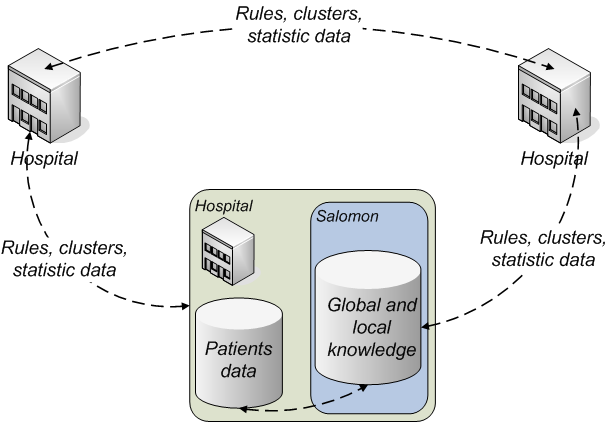
\includegraphics[width=0.8\linewidth]{img/hospital_example.png}
%    \caption{Architekura systemu \emph{Salomon}}
    \caption{The architecture of the example}
    \label{fig:example}
\end{figure}

%System reagowa� b�dzie na zdarzenia:
The system will react to events:

\begin{enumerate}
%  \item Bazda danych zosta�a zmieniona wi�cej ni� 20\% W takim przypadku 
%  zostan� podj�te nast�puj�ce kroki:
  \item The database was changed more than the 20\% in such case the 
  following actions will be undertaken:
	  \begin{enumerate}
%		\item Dost�pne regu�y i klastry zostan� sprawdzone na nowych danych i 
%		ewentualnie zostan� ulepszone
		\item Aviable rules and clusters will be checked on new data and ,if necessary,
%		\item Zostan� wygenerowane nowe regu�y i klastry i por�wnane z najlepszymi 
%		obecnie dost�pnymi
		\item New rules and clusters will be generated and compared with the best
		avialiable ones
%		\item Zostan� wygenerowane nowe dane statystyczne
		\item New statistic data will be generated
%		\item Je�li rezultatem powy�ych krok�w b�dzie uzyskanie lepszej wiedzy, 
%		zostanie ona rozes�ana do reszty w�z��w
		\item If a better knowledge is a result of the above-mentioned steps, it will be
		sent out up to other nodes
      \end{enumerate}
%	\item Inny w�ze� wygenerowa� now� wiedz�
	\item The different node generated the new knowledge
		\begin{enumerate}
%		  \item Wiedza z innego agenta zostanie przetestowana na lokalnych danych
		  \item The knowledge in a different agent will be tested on local data
%		  \item Je�li wynik test�w jest zadawalaj�cy, wiedza ta zostanie ulepszona
%		  korzystaj�c z lokalnych danych
		  \item If the result of tests is satisfactory, the knowledge will be improved
		  using local data  %!! nie wiem czy cos takiego jest mozliwego
		  % wiedza z innego wezla zostanie sumowana z lokana wiedza po czym rezultat
		  % zostanie oceniony
%		  \item W przypadku otrzymania lepszych reg�, klastry zostana zaktualizowane
		  \item In case of obtained better rules, clusters will be updated
		  %\item Wiedza statystyczna zostanie zaktualizowana
		  \item The statistical knowledge will be updated
%		  \item Podobnie jak w przyadku pierwszego zda�enia, je�li powy�sze kroki
%			wygeneruj� dostaniecznie lepsz� wiedz�, zostanie ona rozes�ana do pozosta�ych
%			w�z��w.
		  \item As in case of the first event, if above-mentioned steps generate knowledge which is good
		  enough, it will be sent out to another nodes.
		\end{enumerate}
\end{enumerate}

%Dzi�ki takiej architekturze mogliby�my otrzyma� system kt�ry:
Thanks to such architecture, we gained a system, which:
\begin{enumerate}
%  \item Zapewnia bezpiecz��stwo danych dla ka�dego agenta
  \item Provides data security for every agent
%  \item Ilo�� przysy�anych danych jest zminimalizowana
  \item Minimizes the amount of sent data
%  \item System reaguje na zdarzenia, zatem skomplikowane obliczenia wykonywane
%  s� tylko w przypadku powstania nowych danych lub nowej wiedzy
  \item Reacts to events, and so computing occurs only in case of the
  uprising of new data or the new knowledge being generated
%  \item Ka�dy w�ze� opr�cz og�lnej (najbardziej odpowiadaj�cej wszystkim w�z��)
%  wiedzy, posiada tak�e wi�dz� specyficzn� dla swoich danych
  \item Every node apart from general (the most suitable to all nodes) of 
  knowledge, has also knowledges unique to its data
%  \item Mo�liwo�� zastosowania r�nych algorytm�w i r�nej ich konfiguracji dla
%  ka�ego agenta z osobna
  \item Possibility of applying different algorithms and of their different 
  configuration for every agent individually
%  \item System \emph{Salomon} mo�na zainstalowa� w �rodowisko heterogenicznym.
%  Ka�da plac�wka mo�e posiada� inny system bazodanowy (np. inny schemat bazy
%  danych).
%  Algorytm przekszta�ci�by r�nie zapisane dane do postaci jednolitych
%  atrybut�w.
  \item System \emph{Salomon} it is possible to become installed into 
  heterogeneous environments. Every institution can have a different database system (e.g.
  different database schema). By using attributes, the knowledge could be
  distributed among nodes. The algorithm would convert data differently saved to the figure
  of uniform attributes.

%  \item Obliczenia nie s� scentralizowane. W ka�dej chwili mo�na dodawa� nowych
%  i usuwa� stary agent�w.
  \item Calculations are not centralized. At any time, it is possible to add new
  or to remove old of agents.
\end{enumerate}

% obliczenia nie sa scentralizowane w ka�dej chwili mo�nda dodawa� nowe i usuwa�
% stare w�z�y

%Jak wida� na powy�szym przyk��dzie, \emph{Salomon} �wietnie nadaj� si� do
%rozwi�zywania skomplikowanych i rozproszonych oblicze�. Pozwalaj�c przy tym na
%minimalizacje wysi�ku oraz zasob�w. Nowa wersja platformy ma zawiera� te
%udogodnienia, kt�r� s� niezb�dn� do realizacji tego zadania. Jednak potrzebne s�
%tak�e odpowiednie wtyczki, kt�re dostarcza�by odpowiednich algorytm�w.
As can seen on above example, \emph{Salomon} is fit for solving
complicated and distributed computation. It allows for  
minimizations of effort and resources usage. An updated version of
the platform is supposed to contain these conveniences, which are necessary for the 
realization of this objective. However appropriate plugs, which provide
algorithms, are also needed.


\section{Podsumowanie}
%\subsection{Aktualny stan prac}
\emph{Salomon} nadal znajduje si� w bardzo wczesnym etapie rozwoju.
Nie mo�e by� wykorzystywany w �rodowisku produkcyjnym. Jednak ju� na obecnym poziomie
wykorzystanie \emph{Salomona} do tworzenia drzew decyzyjnych zosta�o zako�czone sukcesem.
To przyk�adowe zastosowanie pozwoli�o udowodni�, �e zaproponowana architektura z powodzeniem,
mo�e by� zastosowana w tego typu zagadnieniach.

\subsection{Przysz�e prace}
Do g��wnych zada� na przysz�o�� nale��:
\begin{itemize}
	\item Dodanie wsparcia dla mechanizmu skaut�w. \\
	
	Obecnie w systemie mo�e zosta� odpalona pojedynczy zestaw zada� jednocze�nie.
	Lista tych zada� zostanie zamieniona grafowym modelem przep�ywu wiedzy i danych
	i mo�liwe b�dzie definiowanie wielu na raz dzia�aj�cych graf�w zada�, kt�re b�d� reagowa�
	na zdarzenia, takie jak, przyk�adowo, pojawienie si� nowych danych w zewn�trznej bazie danych.
	
	\item Wsparcia dla innych typ�w wiedzy poza drzewami. \\
	
	W nast�pnej kolejno�ci, chcieliby�my doda� wsparcie dla regu�.
	
	\item Rozszerzenie wykorzystania rozproszonej architektury.
	
	Poszczeg�lne instancje komunikuj� si� ze sob�, jednak�e brakuje mechanizmu zapewniaj�cego
	najbardziej optymalne rozdzielenie zada�.
	
	\item Dodanie wsparcia dla innych �r�de� danych (wsparcie dla bazy \emph{Firebird}, r�wnie� nie jest kompletne)
\end{itemize}


%\subsection{Przysz�e prace}
%\subsection{Ewentualne zastosowania}
%Do najwa�niejszych przysz�ych pot�cialnych zastosowana� nale�y zaliczy� pomo
%\begin{itemize}
%	\item co zrobiono
%	\item zalety
%	\item braki
%	\item przyszle prace
%	\item ewentualne zastosowania
%\end{itemize}
\newpage

\begin{thebibliography}{99}
\bibitem {bib2} {Kaufman, K. and Michalski, R.S., The Development
    of the Inductive Database System VINLEN: A Review of Current
    Research, International Intelligent Information Processing and
    Web Mining Conference, Zakopane, Poland, 2003}

\bibitem {bib3} {Michalski, R.S. and Kaufman, K., Data Mining and
    Knowledge Discovery: A Review of Issues and a Multistrategy
    Approach, Machine Learning and Data Mining: Methods and
    Applications, R. S. Michalski, I. Bratko and M.  Kubat (Eds.), pp.
    71-112, London: John Wiley \& Sons, 1998}

\bibitem {bib4} {Michalski, R.S., Knowledge Mining and Inductive
    Databases: An Emerging New Research Direction, School of
    Computational Sciences, George Mason University, 2004}

\bibitem {yale} {Mierswa, I., Klinkenberg, R., Fischer, S., Ritthoff, O.,
    A Flexible Platform for Knowledge Discovery Experiments:
    YALE -- Yet Another Learning Environment,
    LLWA 03 - Tagungsband der GI-Workshop-Woche Lernen - Lehren - Wissen -
    Adaptivit�t, 2003.}

\bibitem{uci} {Newman, D.J., Hettich, S., Blake, C.L., Merz, C.J.,
UCI Repository of machine learning databases, Irvine, CA, 1998.}

\bibitem {weka} {Witten, I.H., Frank, E., Data Mining: Practical Machine Learning Tools and
Techniques, Morgan Kaufmann, 2005}



\end{thebibliography}


%wylaczenie numerowania na I stronie
\thispagestyle{empty}


\end{document}
